\chapter{Introduksjon}
\label{ch:introduction}
Hensikten med dette forskningsprosjektet er å evaluere ny teknologi for avstandsoppfølging av kronisk
syke i form av en første prototype av et skytilkoblet pulsoksymeter. Prototypen
vil vises fram for prosjektledere og forskere innen velferdsteknologi for
å avdekke hva som vil bli viktige aspekter ved utviklingen av helseprodukter
basert på \gls{iot}-skyløsninger i fremtiden.
Det overordnete forskningsspørsmålet er: «\fs{}»
Velferdsteknologiprogrammet i Trondheim kommune og SINTEF bistår prosjektet.
Trondheim brukes som eksempelkommune på hvordan avstandsoppfølging prøves ut i starten av 2017.

Dette kapittelet beskriver bakgrunnen for forskningsprosjektet: hva som motiverer det,
forskningsspørsmålene som skal besvares og forskingsdesignet som understøtter det,
hvilke begrensninger og avveininger som er gjort og til slutt en disposisjon av oppgaven.

\section{Bakgrunn og motivasjon}
\textquote[\cite{itu_iot}]{\Acrfull{iot} er en global infrastruktur for informasjonssamfunnet som muliggjør avanserte tjenester ved å
knytte ting sammen fysisk og virtuelt, basert på eksisterende og kommende kompatible informasjon- og kommunikasjonsteknologier}{.}
\gls{iot} gir nye og spennende muligheter for kreative løsninger på problemer på forskjellige områder, alt fra husholdningsapparater
og fjernoppdatering av programvare i biler, til oppfølging av helseproblemer innen velferdsteknologi. Datakraft- og lagring
har blitt mye billigere, noe som gjør at man i større grad enn tidligere kan samle inn informasjon om verden rundt oss
med sensorer. De to største leverandørene av skytjenester, \gls{aws} og Microsoft Azure,
har i løpet av det siste halvannet året lansert nye tjenester for å få sensorenheter tilkoblet til Internett
på en enkel og sikker måte \citep{aws_announcement} \citep{azure_announcement}.

Velferdsteknologi har vært høyt prioritert av helsemyndighetene i Norge de siste årene. Trondheim kommune prøver ut
et prosjekt med avstandsoppfølging av kronisk syke kalt HelsaMi+ på oppdrag fra Helsedirektoratet. 
Avstandsoppfølging kan øke trygghetsfølelsen for innbyggerne og føre til lavere kostnader og færre sykehusinnleggelser.
Løsningen til Trondheim kommune innebærer bruk av et nettbrett der man daglig svarer på spørsmål om hvordan formen er
(figur \ref{fig:intro_helsami}). Noen av pasientene
kan måle vekt, blodtrykk, pulsfrekvens og oksygenmetning ved hjelp av sensorer koblet til nettbrettet.

\begin{figure}
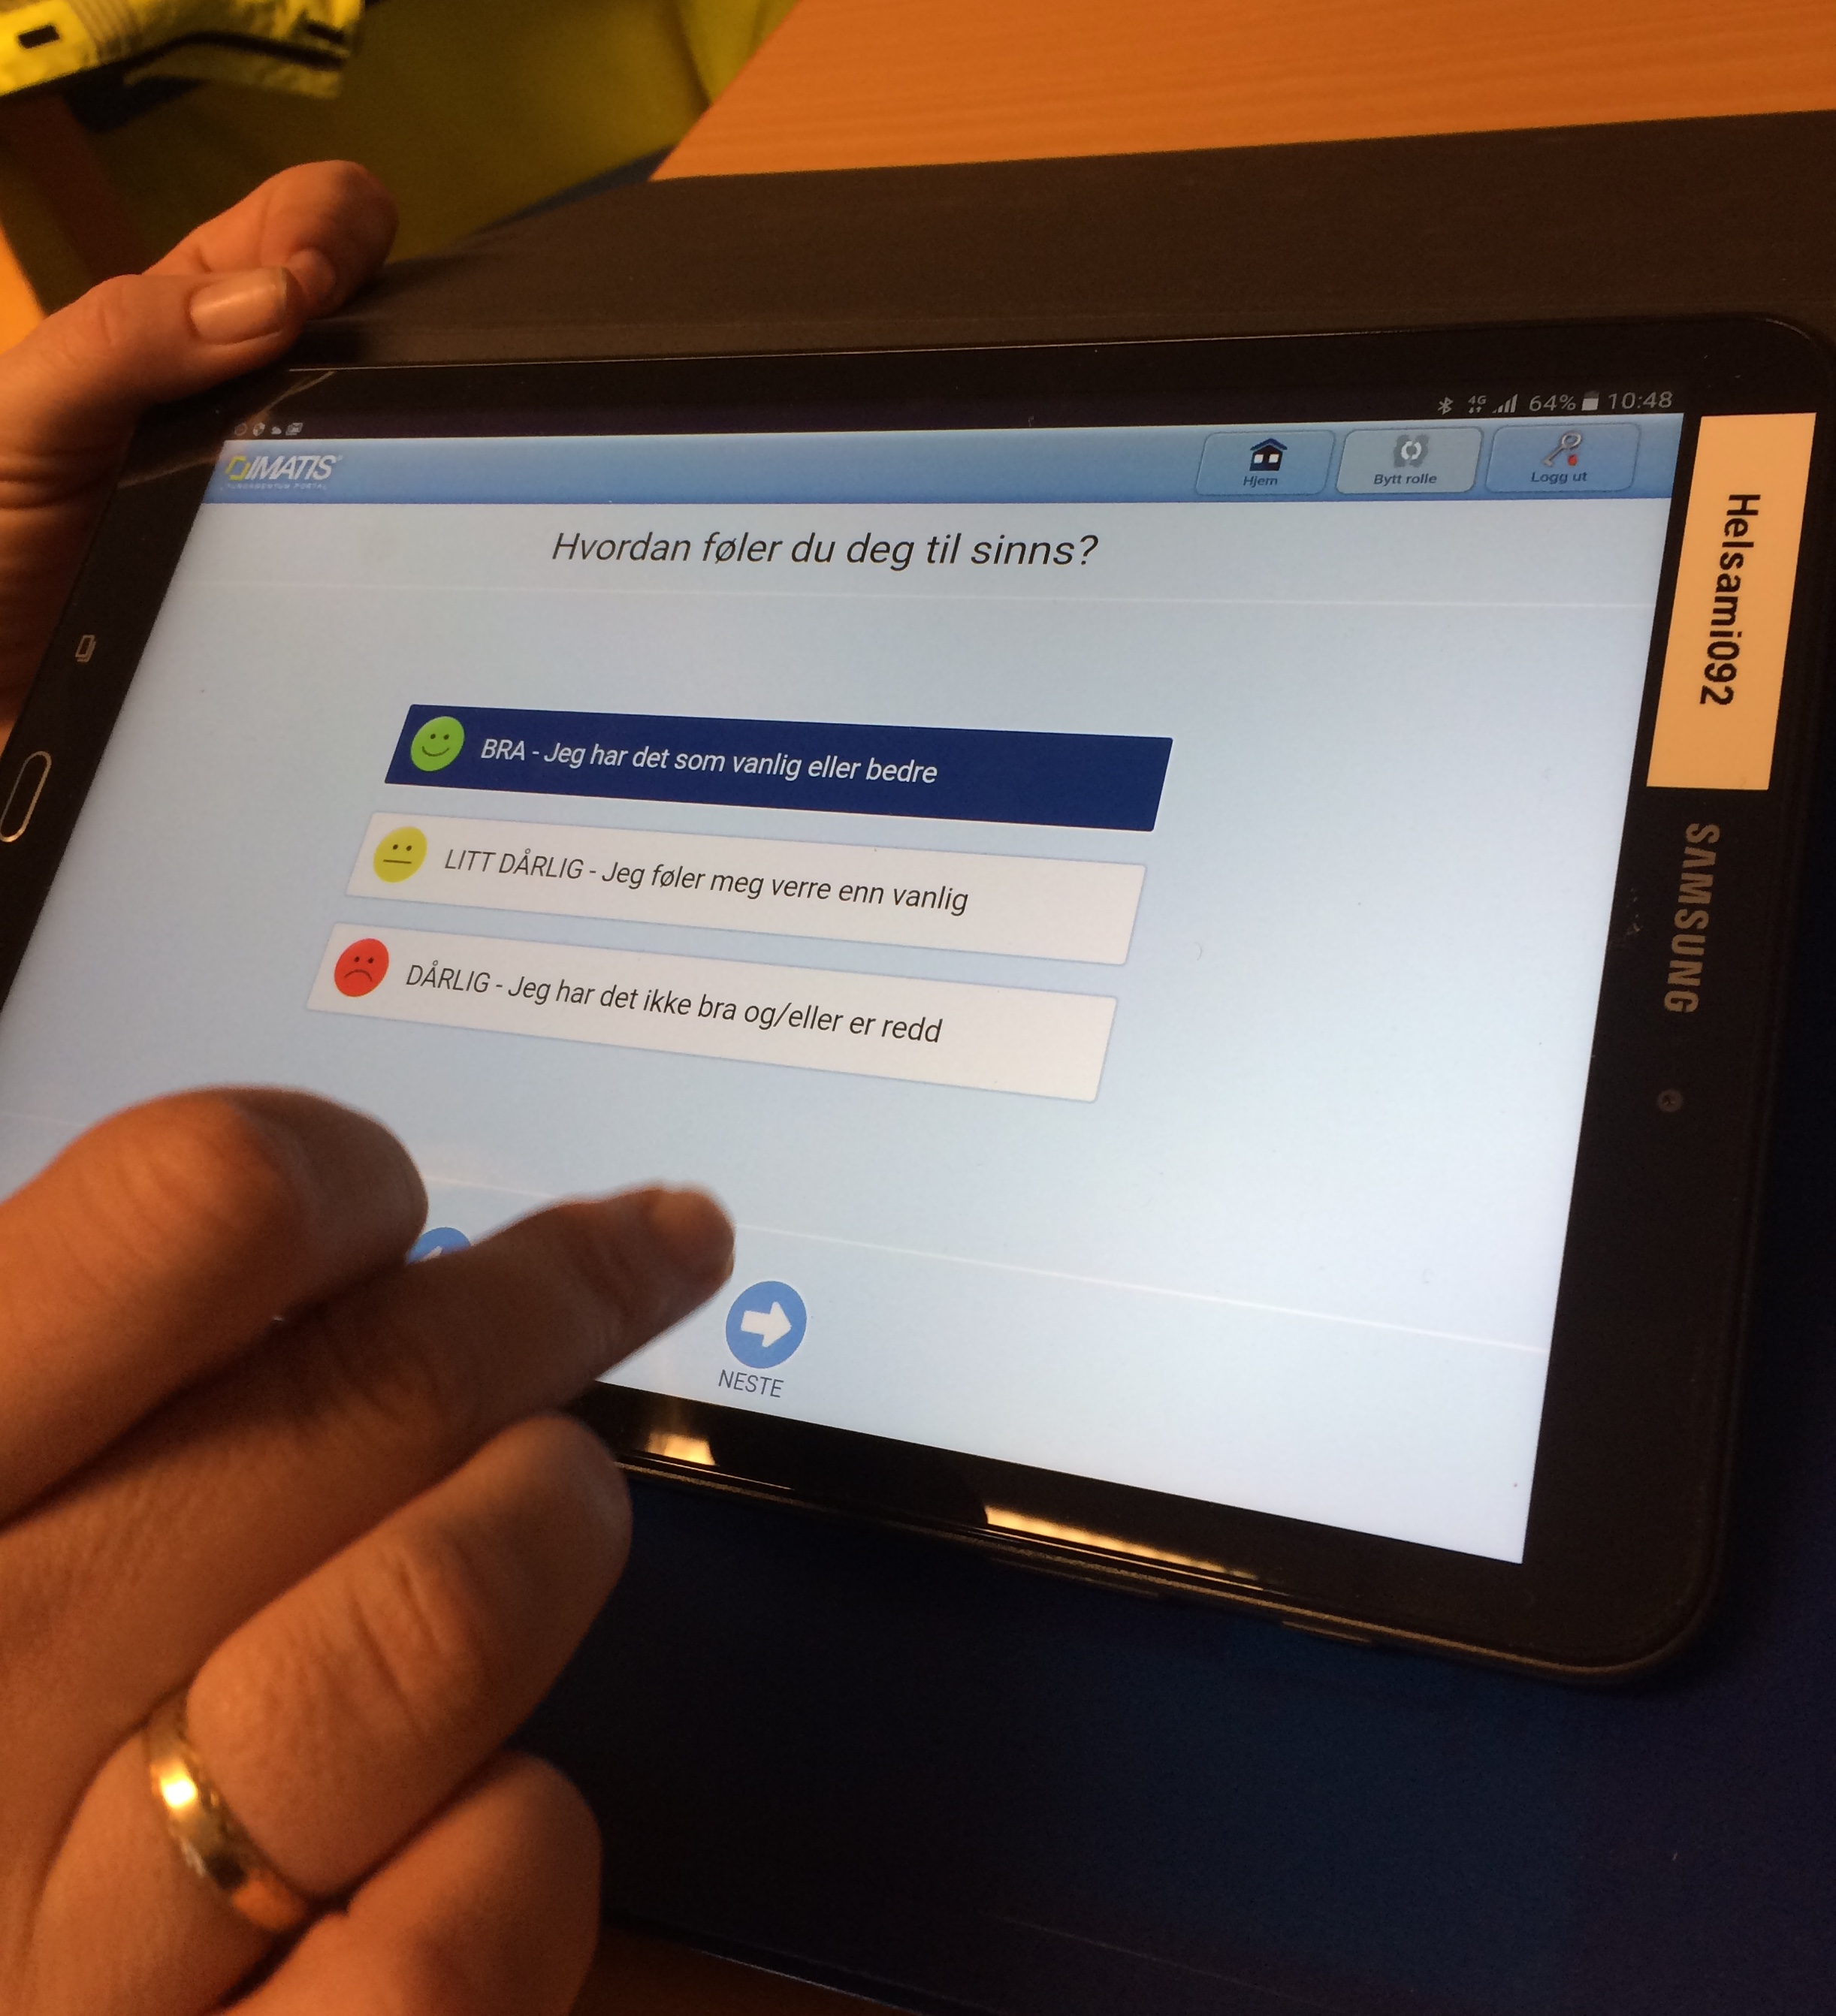
\includegraphics[width=0.7\textwidth,center]{fig/intro_helsami}
\caption{Bruk av nettbrett i HelsaMi+}
\label{fig:intro_helsami}
\end{figure}

Tidligere prosjekter som KOLS Heim har også undersøkt hvordan en bedre kan behandle kroniske pasienter hjemme, og få til økt grad
av samarbeid mellom sykehusene og den kommunale helsetjenesten. KOLS Heim gikk fra 2008 til 2011,
og målet var at \textquote[\cite{kols_idamille}]{(...) bedre samhandling skal kunne
bedre pasientens behandlingstilbud, helsetilstand og livskvalitet, øke kunnskapen om KOLS innen hjemmetjenesten og forhindre
hyppige sykehusinnleggelser}{.} Masteroppgaven «Alternativer for registrering av
pasientopplysninger i hjemmetjenesten» sammenlignet tre ulike teknologier for KOLS Heim: digital penn og papir, PDA/mobiltelefon
og laptop (figur  \ref{fig:intro_gammelkols}).
Der ble digital penn og papir foretrukket \citep{kols_solberg}. Mye har skjedd i den digitale utviklingen siden den gang,
avstandsoppfølging blir dermed en naturlig etterfølger til arbeidet og forskningen som er gjort tidligere.

\begin{figure}
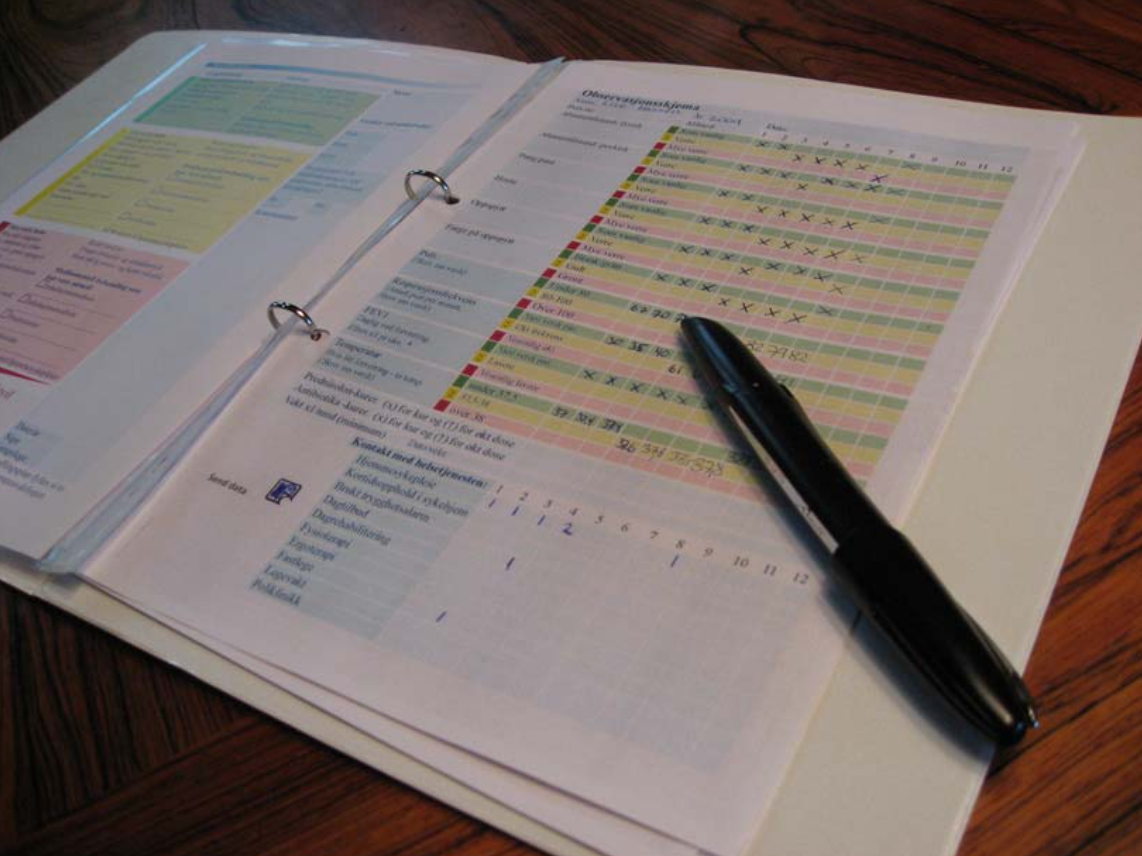
\includegraphics[width=0.7\textwidth,center]{fig/intro_gammelkols}
\caption{Bruk av digital penn \citep{kols_solberg}}
\label{fig:intro_gammelkols}
\end{figure}

Med avstandsoppfølging følger det med seg en rekke utfordringer knyttet til sikkerhet, autentisering, samhandling,
teknologi og brukervennlighet. Hvordan ivaretar man sikkerheten og personvernet til brukeren på en brukervennlig måte?
Dette er krav som skybasert \gls{iot} allerede delvis løser, eller må løse. Mulighetene er store for denne teknologien
med en ny infrastruktur for ting koblet sammen istedenfor infrastruktur for datamaskiner. Prosjektet vil derfor gjøre en utforsking
av tinginfrastrukturen rettet mot helseområdet.

Motivasjonen for forskningsprosjektet er å ta i bruk den nye skyteknologien fra \gls{aws} i en frittstående
pulsoksymeterprototype for avstandsoppfølging av kronisk syke som et alternativ til den løsningen Trondheim
kommune tester ut i dag. Prosjektet vil undersøke hvordan teknologien kan hjelpe til med å understøtte tjenesten som testes ut,
og om den kan avlaste noen av utfordingene kommunen opplever i dag.

Utviklingen av en ny og frittstående prototype gjør at dette prosjektet kan sammenligne de to løsningene og undersøke hvordan ny
teknologi kan brukes i avstandsoppfølging av kronisk syke. Et pulsoksymeter er en sensor som kan måle pulsfrekvens og oksygenmetning i blodet. 

\section{Forskningsspørsmål}
\label{sec:res_questions}
Skybasert \gls{iot} blir presentert som en teknologi som skal løse en mengde problemer knyttet til sensorer. Hvis dette
er sant, så vil det forenkle utviklingen av systemer fordi man kan nyttiggjøre seg ferdig infrastruktur og komponenter. Allikevel
er det få systemer som baserer seg på teknologien. Det er et åpent forskningsspørsmål om teknologien kan brukes i helsedomenet
som har mange komplekse problemstillinger. Avstandsoppfølging passer godt inn som et praktisk eksempel, og utifra lovnadene har
skybasert \gls{iot} potensiale til å forenkle utviklingen i stor grad. Det motiverer følgende forskningsspørsmål:

\begin{enumerate}
    \item[\textbf{FS1}] \fs{1}
    \item[\textbf{FS2}] \fs{2}
    \item[\textbf{FS3}] \fs{3}
    \item[\textbf{FS4}] \fs{4}
\end{enumerate}

Heretter vil «avstandsoppfølging av kronisk syke» bli betegnet som «avstandsoppfølging». Brukere av tjenesten vil
som oftest bli betegnet som «brukere», men i noen tilfeller kan det bety det samme som «pasient».

\section{Forskningsmetoder og forskningsdesign}
Rammeverket for å beskrive forskningsprosjektet er hentet fra \citet{oates}. Hovedstrategien for å besvare på \textbf{FS1} i
delkapittel \ref{sec:res_questions} er å gjøre en liten case-studie på hvordan avstandsoppfølging foregår i Trondheim kommune. Datagenereringsmetoder
er intervjuer og dokumenter. 

For å svare på \textbf{FS2} og \textbf{FS3} vil den primære strategien være \textit{design og kreasjon} (prototyping/\textit{proof of concept})
med intervjuer og dokumenter som datageneringsmetode. Case-studien vil også hjelpe til med å besvare disse spørsmålene. \textbf{FS4} vil drøftes kvalitativt 
utifra svarene på de andre forskningsspørsmålene. Det vil kun gjøres kvalitative dataanalyser.

Forskningsmetodene og forskningsdesignet er utdypet i kapittel \ref{ch:method} og \ref{ch:design}.

\section{Avgrensning av forskningen}
Om man kan gjøre kliniske vurderinger basert på sensordataene, kommer ikke til å være i søkelyset for dette prosjektet,
men vil drøftes kort i kapittel \ref{ch:case} med kommentarer fra en fastlege. Det er noe som kunne vært ytterligere problematisert i en annen oppgave.
Denne forskningen kommer til å anta at det er nyttig å samle inn helsedata fra sensorer for å kartlegge helsetilstanden til kroniske pasienter.

Prototypen gjennomgår ikke brukbarhetstesting. En annen tilnærming til oppgaven kunne vært å gjennomføre brukertester på pasienter eller andre brukere, men det
fører med seg krav om behandling av sensitive helseopplysninger. % @TODO: Dag: Mer i kap x....

Det vil også være umulig å ta hensyn til alle krav og regelverk i helsesektoren ved implementasjonen av prototypen og skyløsningen. Målet vil heller
være å se hvordan teknologien kan understøtte de utfordringene som blir observert innenfor avstandsoppfølging og hvilke muligheter ny teknologi kan gi.

\section{Deltakere i prosjektet}
Fra Trondheim kommune sin side er Ingar Børre Sandvik (prosjektleder, HelsaMi+, program for velferdsteknologi) og
og en som jobber med velferdsteknologi involert (N.N.). Kommunen låner ut et pulsoksymeter.

SINTEF bidrar til forskningsprosjektet. SINTEF gjør mye forskning på
avstandsoppfølging, og bidro også til å få i gang et samarbeid med Trondheim kommune.
To forskere fra SINTEF var med på evaluering- og oppsummeringsintervju der prototypen
ble vist fram.

Terje Røsand (overingeniør, institutt for datateknologi og informatikk) bistår med teknisk hjelp til prototyping og 3D-printing.

Alle aktørene er gjort kjent med formålet for forskningsprosjektet og hva den innsamlede dataen skal brukes til. De er informert om at
intervjuene tas opp på telefon. De har fått tilbud om å lese gjennom transkriberingen av intervjuene og signert
samtykkeerklæringer.

\section{Disposisjon av oppgaven}
Neste kapittel gir en teoretisk bakgrunn innenfor velferdsteknologifeltet og avstandsoppfølging av kronisk syke spesielt.
Det inneholde også bakgrunn om eldres bruk av teknologi, personvern, \gls{iot} og bruken av \gls{iot} i velferdsteknologi.

Kapittel \ref{ch:method} redegjør for forskningsmetodene som brukes i prosjektet, og \ref{ch:design} beskriver hvilket forskningsdesign som brukes i prosjektet for å besvare forskningsspørsmålene.
%Sistnevnte kapittel inneholder også en drøfting om hvorvidt forskningsmetodene er hensiktsmessige, og hva troverdigheten og påliteligheten til forskningsfunnene er.

Kapittel \ref{ch:case} handler om avstandsoppfølging i Trondheim kommune som en case-studie. Det baserer seg på intervjuer gjort med
prosjektleder og en ansatt i Trondheim kommune og skjermbilder av løsningen.

I kapittel \ref{ch:requirements}, drøftes kvalitetskrav til en frittstående \gls{iot}-løsning til bruk i avstandsoppfølging basert på de tidligere
kapitlene.

Kapittel \ref{ch:technology} går igjennom teknologi som er relevant for implementasjonen av et frittstående og skytilkoblet pulsoksymeter,
før kapittel \ref{ch:implementation1} går i detalj på hvordan prototypen ble laget og hvordan den ble seende ut.

Evalueringen av prototypen skjer i kapittel \ref{ch:evaluation1}, der resultatene av intervjuene gjort hos SINTEF og Trondheim kommune oppsummeres.

Avslutningsvis omhandler kapittel \ref{ch:discussion} diskusjon og drøfting av resultatene fra evalueringene, og konklusjonen i kapittel \ref{ch:conclusion}
oppsummerer funnene i oppgaven med bakgrunn i forskningsspørsmålene, med en del om videre arbeid.
